
\usetikzlibrary{arrows.meta,automata,positioning}

\begin{frame}[fragile,label=noBt]{avoiding backtracking?}
\lstset{
        style=small,
        language={},
        moredelim={**[is][\btHL<2|handout:0>]{@hi2@}{@endhi@}},
        }
\begin{lstlisting}
fox  {...}
foo  {...}
off  {...}
.|\n {/* do nothing */}
\end{lstlisting}
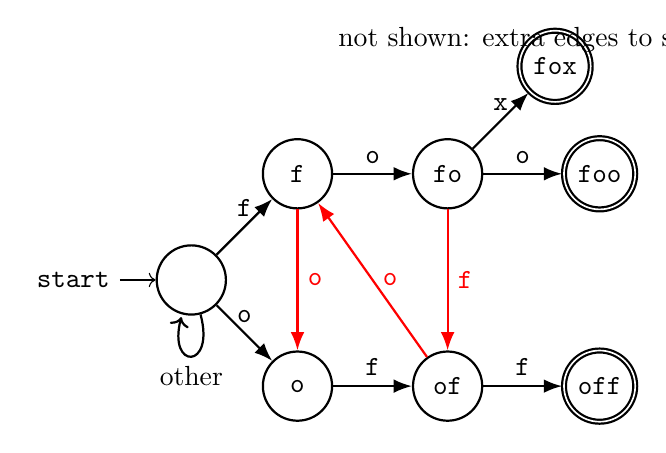
\begin{tikzpicture}
\begin{scope}[every node/.style={font=\tt,thick}]
\node[initial, state,below=2cm,font=\normalfont\it] (start) {};
\node[state,above right=1cm of start] (f) {f};
\node[state,right=1cm of f] (fo) {fo};
\node[state,above right=1cm of fo,accepting] (fox) {fox};
\node[state,right=1cm of fo,accepting] (foo) {foo};
\node[state,below right=1cm of start] (o) {o};
\node[state,right=1cm of o] (of) {of};
\node[state,right=1cm of of,accepting] (off) {off};
\end{scope}
\path[-Latex,thick]
                    (start) edge[loop below] node[below] {other} (start);
\path[-Latex,thick]
                    (start) edge node[above] {\tt f} (f)
                    (f) edge node[above] {\tt o} (fo)
                    (fo) edge node[above] {\tt o} (foo)
                    (fo) edge node[above] {\tt x} (fox)
                    (start) edge node[above] {\tt o} (o)
                    (o) edge node[above] {\tt f} (of)
                    (of) edge node[above] {\tt f} (off);
\path[red,-Latex,thick] (f) edge node[right,align=left] {\tt o} (o);
\path[red,-Latex,thick] (of) edge node[right,align=left] {\tt o} (f);
\path[red,-Latex,thick] (fo) edge node[right,align=left] {\tt f} (of);
\node[overlay] at (fox.north west) {not shown: extra edges to start};
\end{tikzpicture}
\end{frame}

